\problemname{Quicksand}
\noindent

Sandra has moved to Sandsvall to study. After spending a few days in the new town, Sandra
has noticed that there is quicksand in some places. If you go to one of these places, you 
will get stuck in the sand and cannot leave. Sandra wants to know exactly where the quicksand
is, so that she can avoid those places. Fortunately, unlike Gothenburg, Sandsvall has a functioning 
travel-planning app. With the help of this app, Sandra was able to find how long it takes to 
travel from her home to each of the other places in town.

Sandsvall can be represented by an undirected graph with $N$ vertices and $M$ edges.
Sandra's home is located at vertex $1$. It takes one minute to travel between a pair of 
vertices that are connected with an edge. An unknown set of vertices have quicksand, and 
it is not possible to travel from these vertices even if there are edges going to other vertices.

You are given the numbers $d_1, d_2, \dots, d_N$, where $d_i$ is how many minutes it takes to travel from 
vertex $1$ to vertex $i$. If it is impossible to travel to vertex $i$ at all, then $d_i = -1$.
Your task is to find which vertices have quicksand, with the help of this information.

\section*{Input}

The first line contains two integers $N$ and $M$ ($2 \leq N \leq 3 \cdot 10^5$, $N-1 \leq M \leq 3 \cdot 10^5$).

The second line contains the $N$ integers $d_1, d_2, \dots, d_N$ ($-1 \leq d_i \leq N$). The first number 
$d_1$ will always be zero.

The following $M$ lines contain two integers $u_i, v_i$ ($1 \leq u_i, v_i \leq N$, $u_i \neq v_i$), which means 
that there is an edge between $u_i$ and $v_i$. There will be at most one edge between each pair of vertices.
The graph will always be connected, which means that it is possible to reach every vertex
via a sequence of edges (but the quicksand can make it so that some vertices are unreachable).

\section*{Output}

If there is no possible way for the quicksand to be distributed that corresponds with 
the given information, print $-1$.

Otherwise, first print an integer $K$ ($0 \leq K \leq N$), the number of vertices that have quicksand.
Then, print $K$ different integers $a_1, a_2, \dots, a_K$, the indices of the vertices that have quicksand.
If there are many possibilities, you can print any of them.

\section*{Scoring}
Your solution will be tested on a set of test groups, each worth a number of points. Each test group contains
a set of test cases. To get the points for a test group you need to solve all test cases in the test group.

\noindent
\begin{tabular}{| l | l | p{12cm} |}
  \hline
  \textbf{Group} & \textbf{Score} & \textbf{Constraints} \\ \hline
  $1$    & $17$        & The graph is a line, i.e. $M = N-1$ and the edges are $(1, 2), (2, 3), \dots, (N-1, N)$\\ \hline
  $2$    & $29$        & The graph is a tree, i.e. $M = N-1$. \\ \hline
  $3$    & $34$        & The answer is never $-1$. \\ \hline
  $4$    & $20$        & No further constraints. \\ \hline
\end{tabular}

\section*{Sample explanation}

\begin{figure}[h!]
  \centering
  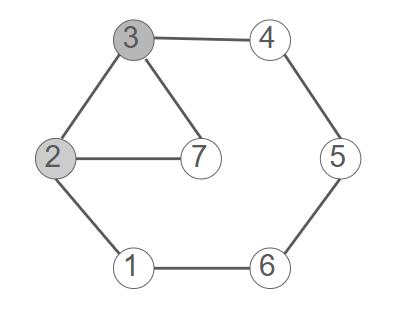
\includegraphics[width=0.3\textwidth]{kvicksand.PNG}
  \caption{The graph in sample 1}
\end{figure}

In sample 1 it is possible that vertices $2$ and $3$ have quicksand, as the image shows.
For example, that would make vertex $7$ impossible to reach. Vertex $7$ could also have quicksand, 
so another possible answer is $2,3,7$.
